\documentclass{config/apuntes}

\title{Minería de Textos}
\author{Sandra Mingo Ramírez}
\date{2025/26}
\acronym{AIBM}

\usepackage[all]{nowidow}
\usepackage{listing}
\usepackage{color}
\usepackage{tabularx}
\usepackage{multirow}
\usepackage{makecell}
\usepackage{amsmath}
\usepackage{array}
\usepackage{soul}

\definecolor{dkgreen}{rgb}{0,0.6,0}
\definecolor{gray}{rgb}{0.5,0.5,0.5}
\definecolor{mauve}{rgb}{0.58,0,0.82}

\lstset{
  frame=tb,
  aboveskip=3mm,
  belowskip=3mm,
  showstringspaces=false,
  columns=flexible,
  basicstyle={\small\ttfamily},
  numbers=none,
  numberstyle=\tiny\color{gray},
  keywordstyle=\color{blue},
  commentstyle=\color{dkgreen},
  stringstyle=\color{mauve},
  breaklines=true,
  breakatwhitespace=true,
  tabsize=3
}

\usepackage{tocloft}

\advance\cftchapnumwidth 0.9em\relax
\advance\cftsecnumwidth 0.6em\relax
\advance\cftsubsecindent 0.5em\relax
\advance\cftsubsecnumwidth 0.5em\relax
\begin{document}

\begin{abstract}
La minería de textos, también conocida como minería de datos de texto, es el proceso de transformar texto no estructurado en un formato estructurado para identificar patrones significativos y nuevos conocimientos. Puede utilizar la minería de textos para analizar vastas colecciones de materiales textuales para capturar conceptos clave, tendencias y relaciones ocultas.
\end{abstract}

\pagestyle{plain}

\maketitle

\tableofcontents

%20/10 - Kostadin
\chapter{Introducción al lenguaje}
\section{Textos}

Los humanos nos comunicamos principalmente de forma oral, y el texto es la representación escrita de ese habla. Los animales también se comunican, usualmente sobre el estado actual o presente. El texto es una abreviación del habla, una forma de transcribirla con ciertas características:
\begin{itemize}
\item Es muy comprimido: el habla se produce mediante la acción de los músculos controlados por la corteza motora. Estamos limitados a emitir una cadena unidimensional de sonidos o fonemas.
\item Las categorías de sonido están acotadas y corresponden a los morfemas del lenguaje. Al escribir los morfemas, ya tenemos el texto.
\item El texto se transmite a través de letras, símbolos discretos.
\end{itemize}

El texto es una transcripción de una señal sonora que mantiene sus propiedades esenciales. Puede copiarse indefinidamente y es resistente al ruido.

El objetivo de la minería de textos es extraer información relevante de textos escritos. Algunos términos clave son:
\begin{itemize}
\item Información: Una letra es una unidad de información. Un dígito tiene menos opciones (0-9) comparado con las letras (a-z), por lo que posee menos información. Para codificar todo el abecedario se requieren al menos dos dígitos. La cantidad de información depende del número de posibles mensajes. Por ejemplo, con un dígito hay 10 posibilidades, con dos dígitos 100, y con tres dígitos 1000. En informática, se usan dos dígitos binarios (0 y 1). El logaritmo en base 2 mide la información en bits: 
$log_2(3) \approx 10$.
\item Relevancia: Algo es relevante si está relacionado con un problema específico. Por ejemplo, si buscamos una sustancia que cause diabetes en ratones, lo relevante es todo lo que se relacione con esa sustancia. La relevancia depende del problema concreto.
\item Fiabilidad: Debemos trabajar con información fiable, preferiblemente basada en la realidad y datos experimentales.
\item Texto humano: Tiene una estructura que viene de la secuencia continua de movimientos musculares al hablar. Además, existe una estructura jerárquica dada por la gramática y la sintaxis.
\end{itemize}

La redundancia garantiza robustez ante el ruido. El texto es redundante en varios niveles:
\begin{enumerate}
\item Fonemas: un fonema, como la vocal "a", tiene una duración corta (décimas de segundo). Si parte de la señal se pierde, otras repeticiones ayudan a comprenderlo.
\item Variaciones pequeñas en sonidos o escritura normalmente no afectan al significado. Por ejemplo, quitando las vocales, aún podemos entender un texto. Muchos lenguajes antiguos, como el árabe o los lenguajes semitas, no escriben vocales. Estas se introdujeron para facilitar la lectura sin conocer el contexto.
 \end{enumerate}

Ejercicio: estimar la velocidad de transmisión entre humanos de texto en dos contextos: uno escribe y el otro lo recibe; uno lee algo ya escrito como una novela. No se puede estimar la información, solo un límite superior a la información ("no más que x"). %Esto no hay quien lo entienda
\begin{itemize}
 \item Vídeo: 5 000 000 bits por segundo
 \item Teléfono: 3 000 bps
 \item Radio: 20 000 bps
 \item Leer (para uno mismo, en silencio): de media 200 palabras por minuto, unas 1000 letras por minuto. Siendo 6 bits la letra, 6000 bits por minuto o 100 bps.
 \item Escribir un texto: 60-90 palabras por minuto, con una media de 5 letras por palabra: 360-540 letras por minuto. Siendo 6 bits la letra, sale 40-60 bps
\end{itemize}

No toda comunicación es habla humana. Por ejemplo, si una persona describe algo para que otra lo dibuje, la información transmitida será muy diferente.
Tenemos diferentes tipos de señales: sonora o de letras. En términos de información, la función $f(x)$ tiene menos información que su argumento $x$, es decir, $f(x) < x$. 

\section{Artículos}
La mayoría de la información científica se encuentra en artículos. Un artículo es un texto publicado que puede incluir imágenes y fórmulas. Los artículos científicos y periodísticos se parecen: ambos tienen autores y reflejan la opinión de éstos. El artículo es una función de la información del evento, por lo que contiene menos información que el propio evento. Los autores están limitados por sus conocimientos y la fuente de información a la que acceden, como vídeos, relatos, testimonios, etc. El tiempo de escritura es también importante; el autor produce la mejor versión posible en ese momento, dentro de su contexto.

Un artículo de una página de periódico suele tener unas 300 palabras. Este valor puede obtenerse comprimiendo el contexto y el artículo.

En artículos científicos existe cierto grado de censura; no todo lo que sabe el autor se incluye. Cuanto más accesible es el artículo, mejor, por eso existen iniciativas OpenSource. Existen varios tipos de artículos científicos: investigación original, reviews (revisión de varios trabajos), propuestas metodológicas, estudios de caso (case studies, con potencia estadística limitada) y opiniones.

Un artículo cercano a la realidad contiene más información. Las fuentes más fieles incluyen historiales clínicos, diarios de laboratorio, datos estadísticos, comunicaciones entre personas sobre hechos, y datos del Internet of Things.

Actualmente, también están disponibles fuentes preprocesadas por inteligencia artificial (IA), que son modelos estadísticos del lenguaje. Reflejan la opinión prevalente, pero no su diversidad, tienen un horizonte temporal limitado, y un retraso por el tiempo de entrenamiento. Estas fuentes pueden reforzar opiniones dominantes debido a feedback positivo. Por ello, es recomendable complementar búsquedas IA con consultas directas a la web, aunque gran parte de la información en la web también ha pasado por IA.

\section{Minería de datos}
La minería de textos analiza uno o varios textos para responder preguntas como: ¿de qué trata? ¿Es fiable? ¿Tiene interés? ¿Qué información contiene y cómo describirla? ¿Cuál es la información nueva? ¿Cómo presentar la información de forma estructurada?
Los formatos estructurados incluyen bases de datos relacionales, no relacionales, grafos y programas.

Ejercicio: Food Insecurity Interventions to Improve Blood Pressure - JAMA Internal Medicine. 
El artículo tiene información no textual, está en los gráficos. Tiene 458 participantes, que está bien en cuanto a potencia estadística. 

Los \textbf{datos estructurados} tienen organización clara, fáciles de consultar, modificar y analizar, y suelen ser isomórficos con tablas relacionadas. Ejemplos: bases de datos, hojas Excel, gráficos conceptuales, datos de formularios.

Los \textbf{datos no estructurados} carecen de un modelo fijo, están en formatos naturales mezclando información útil con redundante, y no se pueden organizar trivialmente en tablas. Ejemplos: texto, vídeo, imagen.

El hipertexto es texto con relaciones internas o externas. Se estima que el 80\% de los datos son no estructurados.

\begin{figure}[h]
\centering
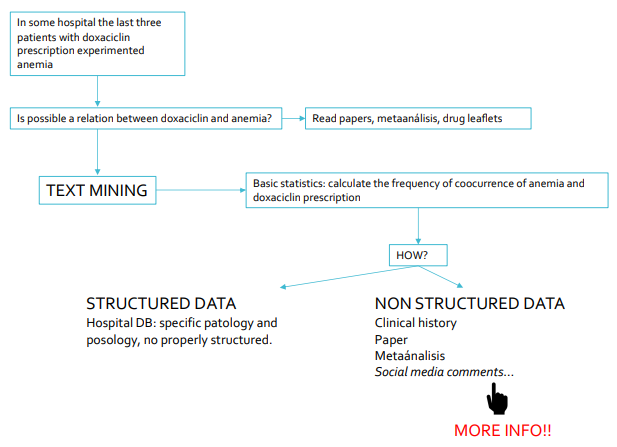
\includegraphics[width = \textwidth]{figs/ej-mineria.png}
\end{figure}

El trabajo fundamental en procesamiento de lenguaje natural es transformar datos no estructurados en estructurados. La idoneidad del método depende de la tarea real.
Dos grandes grupos de métodos:
\begin{itemize}
\item Métodos clásicos: dividir una tarea compleja en subtareas simples (p. ej. sistema de preguntas y respuestas basado en etiquetado POS, análisis sintáctico, reconocimiento de entidades nombradas) y combinarlas para generar la respuesta en lenguaje natural.
\item Métodos basados en aprendizaje profundo: un sistema único que procesa grandes cantidades de texto para crear una representación interna útil a la tarea.
\end{itemize}

\begin{figure}[h]
\centering
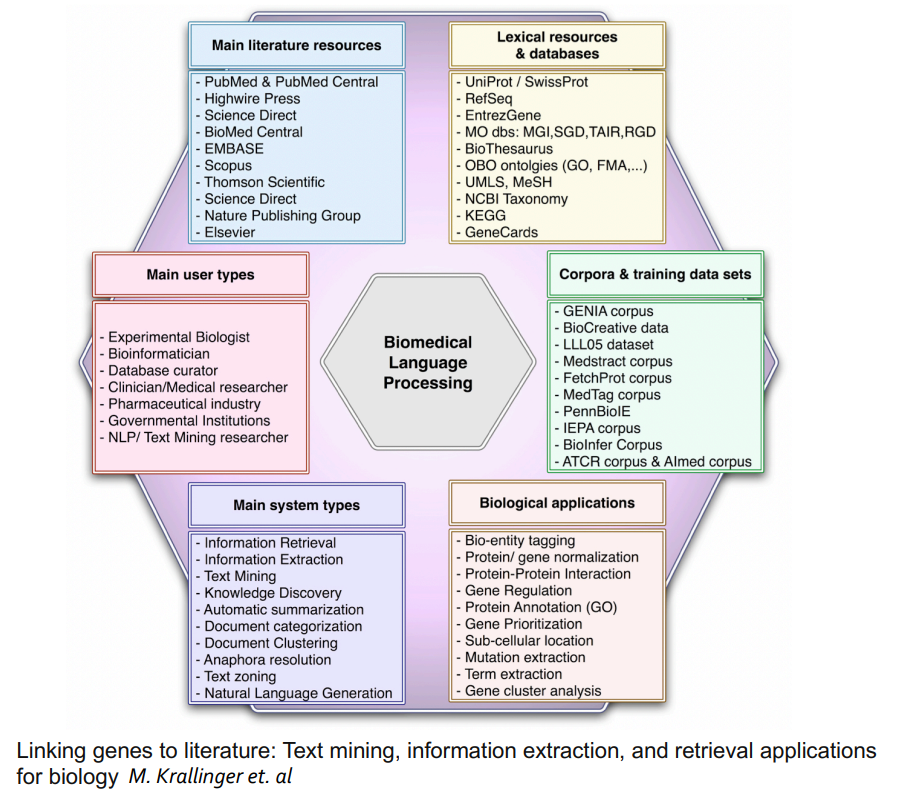
\includegraphics[width = 0.6\textwidth]{figs/blp.png}
\end{figure}

La pipeline del NLP funciona de la siguiente forma:
\begin{enumerate}
\item Extracción de datos de texto: Selección de las fuentes de datos de texto, aplicación de diferentes técnicas de consulta, API REST, extracción de datos web, consulta de bases de datos
\item Preprocesado: Formateo y estandarización de los datos de texto. Incluye tokenización, derivación, eliminación de palabras vacías y corrección gramatical.
\item Transformación de características: Transformación de los datos de texto en características procesables por ordenador.
Codificación N-gram, etiquetado POS, análisis sintáctico, agrupación Brown, vectores de palabras.
\item Generación del modelo
\item Análisis y tratado de resultados: estandarización, almacenamiento de los resultados
\end{enumerate}

\begin{figure}[h]
\centering
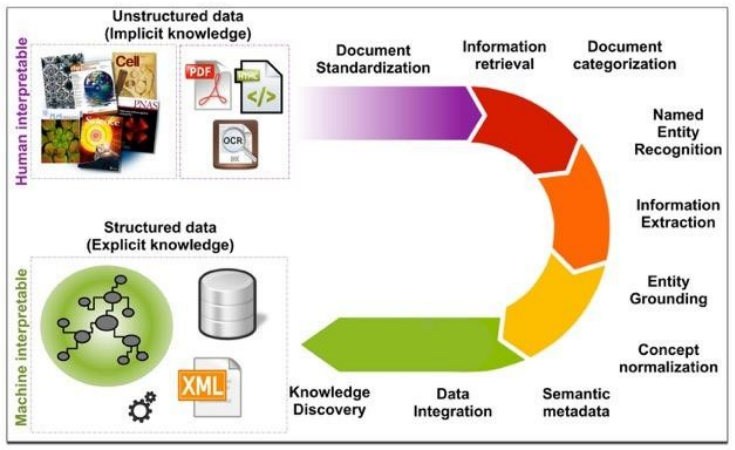
\includegraphics[width = 0.6\textwidth]{figs/biocuration.png}
\end{figure}

La biocuración es el proceso de recogida, verificación, organización y mantenimiento de datos biológicos para asegurar su calidad, coherencia y utilidad. En el contexto de la bioinformática, la biocuración implica seleccionar información relevante, estandarizarla y anotarla correctamente en bases de datos especializadas, facilitando así su análisis y reutilización en investigaciones científicas. El objetivo principal es transformar datos brutos en recursos confiables y estructurados que permitan realizar estudios precisos y reproducibles.

\begin{figure}[h]
\centering
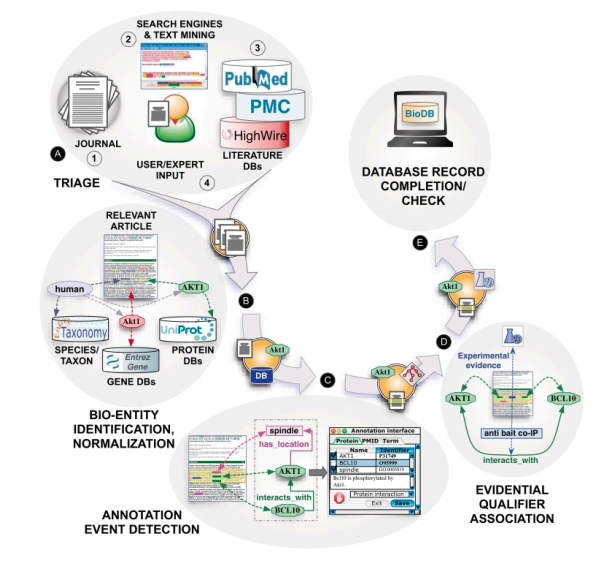
\includegraphics[width = 0.6\textwidth]{figs/biocuration2.png}
\end{figure}

Pese a la ayuda de la IA, la biocuración sigue siendo un proceso manual. Sus pasos son:
\begin{itemize}
\item Triaje: selección de artículos relevantes. El NLP clasifica el texto, detecta las entidades y tiene un aprendizaje no supervisado.
\item Normalización e identificación de bioentidades: hay varios nombres para una  misma patología, síntoma, causa, etc, por lo que se deben marcar como iguales. Por ejemplo: enfermedades vasculares hipertensivas, hipertensión e hipertensión arterial hacen alusión a lo mismo, pero con palabras distintas.
\item Anotación de eventos detectados: interacciones proteína-proteína, producción génica en cuanto a localización celular, etc, extracción de relaciones en general.
\item Asociación de calificadores probatorios
\item Comprobación y completar las entradas de la base de datos
\end{itemize}

Extraer relaciones entre entidades es una de las tareas más difíciles en
bioNLP. Es difícil porque, por un lado, es complicado extraer información significativa de la muestra para construir un modelo automático y, por otro lado, los modelos heurísticos no pueden abarcar todo el espectro de casos.

\subsection{Ontologías}
Más de 1500 bases de datos biológicas activas con datos y términos de diferentes campos y más de 200 vocabularios diferentes incluidos en recursos como UMLS: ontologías genéticas, secuencias genéticas, estructura proteica, terminología médica, taxonomías de especies, etc.

El UMLS (Unified Medical Language System) integra y distribuye terminología clave, normas de clasificación y
codificación, y recursos asociados para promover la creación de sistemas y servicios de información biomédica más eficaces e interoperables, incluidos los registros médicos electrónicos.

Originalmente integró 2 millones de nombres para unos 900 000 conceptos de más de 60 familias de vocabularios biomédicos, así como 12 millones de relaciones entre estos conceptos.
\begin{itemize}
\item Vinculación de términos con diccionarios estándar.
\item Exploración de ontologías de términos.
\item Búsqueda de relaciones entre términos.
\item Correspondencia entre uno y muchos de diferentes fuentes de bases de datos.
\end{itemize}

Los Medical Subject Headings (MeSH) son un vocabulario controlado y organizado jerárquicamente elaborado por la Biblioteca Nacional de Medicina. Se utiliza para indexar, catalogar y buscar información biomédica y relacionada con la salud.


%Exercise (5 min): Look at the repository PMC. Perform a query about the subject of the Jama article. Describe the structure of the query (righthadside window). Poner también la ontología MeSH
%22/10 - Paco Jurado
\chapter{Procesamiento de lenguaje natural}
\section{Procesado de lenguaje natural}
\subsection{Definición de PLN}
El procesamiento del lenguaje natural (NLP por sus siglas en inglés) son un conjunto de métodos para hacer el lenguaje humano accesible a los ordenadores. Así, permite una comunicación "natural" entre humanos y máquinas y mejora la comunicación entre humanos (por ejemplo por traducción).

La ciencia ficción ya mostraba desde finales de los 70 máquinas que podían hablar. 

\subsection{Desafíos del NLP}
El test de Turing lo desarrolló Alan Turing en 1950 para comprobar la capacidad de una máquina a mantener una conversación como si fuera un humano. El test se basa en un humano que "chattea" y debe distinguir si está hablando con otro humano o con una máquina. Si no lo puede distinguir, se considera que la máquina ha pasado el test de Turing. 

NLP es difícil porque los lenguajes humanos son ambiguos, ilimitados, diversos, difusos, más y menos articulados. Hay palabras polisémicas, el orden de las palabras afecta a su significado, expresiones hechas ("dame tu teléfono" no se refiere al dispositivo, si no al número). La ambigüedad sintáctica se puede dar por la sintaxis, referencias a pronombres, y aunque para los humanos sea fácil de detectar y forme la base de muchos chistes, a la hora de pasarlo a la máquina se convierte en un problema. 

A la hora de hacer las traducciones, depende la composición de palabras. Dos palabras que por separado tienen un significado, cuando están juntas pueden tener otro. 

\subsection{Interdisciplinariedad del NLP}
El NLP se basa en muchas disciplinas muy diversas. Están los \textbf{lingüistas}, que buscan analizar cómo funciona el lenguaje, los ingenieros en \textbf{machine learning} e \textbf{inteligencia artificial} para poder automatizar las tareas y crear programas complejos. En general, toda la \textbf{informática} presenta la base de los algoritmos utilizados en NLP.

Estas áreas son las que diseñan los primeros algoritmos, pero con el tiempo salen cuestiones \textbf{sociales y éticas} por sesgos sociales, como pueden ser los géneros al traducir del inglés al español (nurse se traducía sólo como enfermera, no salía la alternativa de enfermero).

\section{Aplicaciones prácticas}
Entre las aplicaciones del NLP se encuentran:
\begin{itemize}
\item Traducción automática: traducción de un texto de un idioma a otro en su significado (no palabra por palabra).
\item Obtención de información: dada una consulta en nuestro idioma, identifica los documentos y páginas relevantes para esa búsqueda. 
\item Extracción de información: se tienen documentos de texto que no están estructurados (en cuanto a información, no del texto) de los cuales se intenta extraer la información estructurada para una base de datos.
\item Respuesta a preguntas: responder automáticamente preguntas propuestas por humanos en base a la información ya almacenada.
\item Clasificación de texto: asigna categorías o tags a textos en base a su contenido.
\item Minería de opiniones y análisis de sentimientos: identificar, extraer, cuantificar y estudiar de forma sistemática los estados afectivos y la información subjetiva (a partir del contenido textual generado por los usuarios).
\item Sistema de diálogo: Un agente conversacional o chatbot es un sistema informático diseñado para conversar con un ser humano (a través de un canal de texto). Los asistentes virtuales/personales inteligentes pueden realizar tareas o prestar servicios a una persona basándose en órdenes o preguntas. Así se crearon los agentes de generación de lenguaje conversacionales como ChatGPT o Gemini. Estos algoritmos generan texto como lo haría un humano (o como se ha hecho previamente), y estos sí pasan el test de Turing.
\end{itemize}

\section{Niveles del análisis lingüístico y tareas NLP}
\subsection{El pipeline de NLP}
Para conocer un idioma, hay que manejar muchos niveles de análisis lingüístico: habla, fonética, ortografía, morfología, lexemas, sintaxis, semántica, pragmática, etc. 

\begin{figure}[h]
\centering
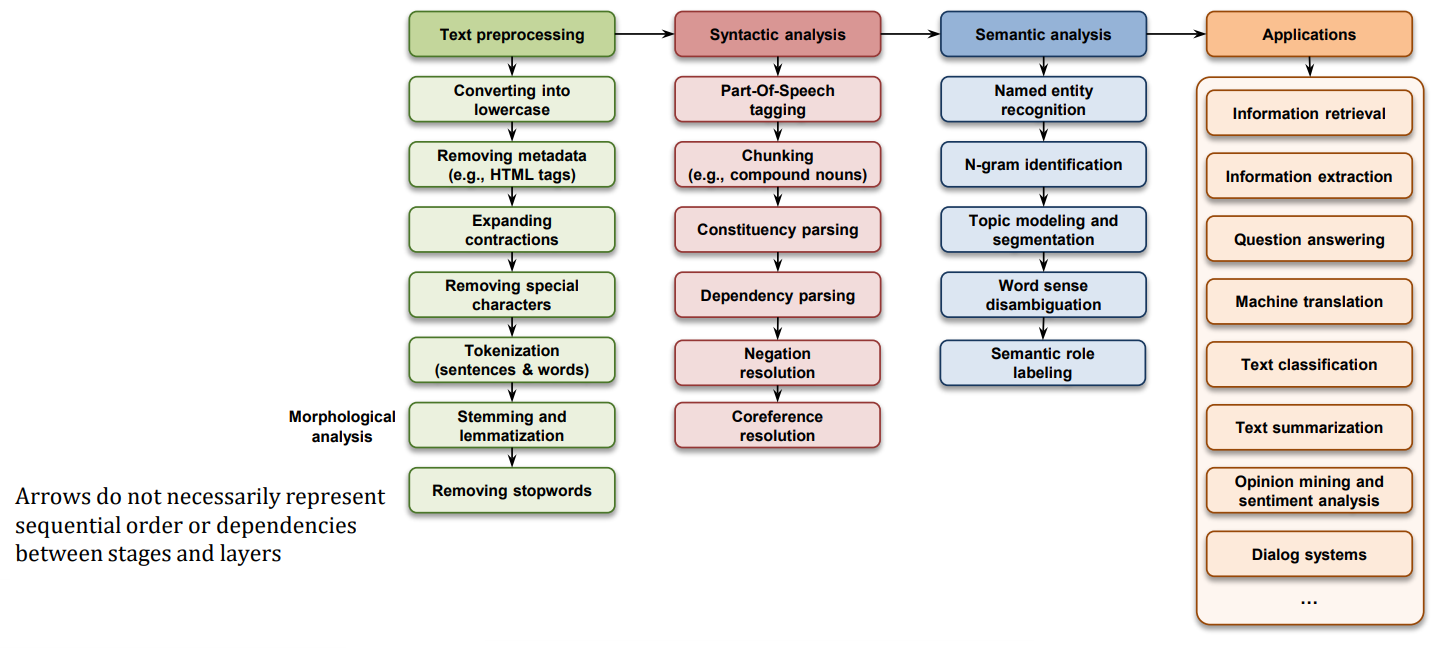
\includegraphics[width = \textwidth]{figs/nlp-pipeline.png}
\end{figure}

El primer paso es el \textbf{preprocesamiento} para normalizar todo (pasar a minúscula), quitar la metadata (tags, html), expandir las contracciones o los acrónimos, eliminar caracteres especiales, etc. También se eliminan las stopwords, que son palabras que no aportan nada de información, como los artículos o los verbos auxiliares. A continuación se stemiza y lematiza, es decir, se quitan las conjugaciones para obtener la raíz y obtener el lema (la palabra normalizada).

El siguiente paso es el \textbf{análisis sintáctico} donde se identifican las partes de la oración, se hace una composición de los grupos (nominales, preposicionales, etc) donde entra el análisis de constituyentes, resolución de dependencias y negaciones y se entra al \textbf{análisis semántico}. Con todo el procesamiento se pasan a las \textbf{aplicaciones}.

\subsection{Análisis sintáctico}
\paragraph{Part-Of-Speech (POS) tagging}
El POS tagging identifica para cada palabra o token si se trata de un nombre propio, verbo, determinante, etc. 

\paragraph{Parseo de constituyentes}
Las palabras tienen su POS tag y se van agrupando las estructuras sintácticas.

\paragraph{Parseo de dependencias}
Se extrae la estructura gramática de una oración, buscando la relación entre los constituyentes definidos previamente. 

\subsection{Análisis semántico}
\paragraph{Named Entity Recognition (NER)}
El reconocimiento de entidades se utiliza mucho en distintos contextos. Busca reconocer localizaciones, personas, lugares geopolíticos, números de teléfono, fechas, etc. Esto se puede utilizar posteriormente para la extracción de información. 

\paragraph{Resolución de co-referencias}
Se busca qué hace referencia a la misma entidad en un texto para reemplazarlo y que el procesamiento del texto sea igual. En ocasiones, es necesario completar la información (por ejemplo, una noticia de "el presidente ha dicho ...", si a la semana hay un cambio de gobierno).

\paragraph{Word Sense Disambiguation (WSD)}
En ocasiones, las palabras pueden hacer referencia a más de una cosa por ser polisémicas o tener otras ambigüedades, por lo que se deben desambigüar. Para ello se debe ver el contexto de la oración. Generalmente, se coge la palabra de la frase con menos alternativas de ambigüedades y a partir de ella se escogen las otras acepciones.

\paragraph{Etiquetado semántico}
Al hacer el etiquetado semántico, se le está poniendo cierta taxonomía para indicar las estructuras predicado-argumento como agente, predicado, tema y localización. Son representaciones abstractas de las funciones.

\section{Breve historia del NLP}
\subsection{NLP antes de la era Deep Learning}
Los inicios se deben a lingüistas y matemáticos. En los 1960s, se formalizan las teorías gramáticas. En los 90 se generan modelos estadísticos que permitieron identificar los stopwords en base a la frecuencia. Los modelos bayesianos funcionaban muy bien.

\subsection{NLP durante la era Deep Learning}
Los primeros modelos neuronales aplicados al lenguaje entraron en el 2003 y requerían una computación enorme. En los 2010 se crearon las GPU, por lo que el tratamiento matricial mejoró con creces. También entraron los word embedding, donde se obtenían representaciones vectoriales de los conceptos vinculados a las palabras con redes neuronales. Esto marcó un antes y un después. Se crearon distintas arquitecturas con los mecanismos de atención y transformer, y en 2020 los modelos grandes de lenguaje.

Muchos de los modelos creados antes de la era Deep Learning se siguen utilizando hoy día. Si por la tarea no se requiere una arquitectura deep, se pueden utilizar los modelos "clásicos". 
%22/10 - Paco Jurado
\chapter{El sentido de las palabras}
\section{Definiciones}
Hay palabras que tienen varios significados. Dado un lema o una palabra sin sus flexiones (en su forma más "normal") salen cada uno de las acepciones y significados. 

Un lema es una forma canónica de las palabras. Se coge la raíz y se añade lo pertinente para añadir el lema. Hay muchos algoritmos para obtenerlos, aunque son dependientes del idioma. Por ejemplo, en inglés se puede eliminar -ed o -ing para obtener el verbo sin conjugar. 

Las glosas son las definiciones. Esto no le sirve al ordenador, solo a nosotros al buscar un lema en el diccionario. 

Los homónimos son palabras que comparten una forma, pero tienen significados distintos. Banco puede ser la institución financiera o el asiento del parque, bat puede ser murciélago o bate. La homonimia se identifica en la extracción de información o question-answering, y viene en función del contexto. 

La polisemia es que una palabra pueda significar varias cosas relacionadas. La metonimia es la polisemia de forma sistemática. Por ejemplo, universidad puede ser el edificio o la institución. 

\section{Relaciones entre acepciones de palabras}
\subsection{Sinonimia y antonimia}
El sinónimo perfecto no existe, suele haber un matiz que los diferencie, ya que si no se hubiese abandonado una de las palabras. Hay veces que el contexto no permite intercambiar dos palabras. Por ejemplo, big y large, pese a ser sinónimos, sólo es correcto big en caso de "big sister". 

Los antónimos tienen significados típicamente opuestos. Ocurre similar que con los sinónimos, habiendo matices que hace que no sean antónimos perfectos. 

\subsection{Hipónimos e hiperónimos}
Los hipónimos son palabras que son más específicas que otras. Por ejemplo, coche es un hipónimo de vehículo, ya que es más específico. Hiperónimo es todo lo contrario, siendo una superclase más genérica. 

\subsection{Meronimia y holonimia}
La meronimia denota una parte de algo, y holonimia lo contrario. Por ejemplo, rueda y coche, u oveja y rebaño.

\section{WordNet}

WordNet es un tesauro o diccionario, una base de datos que representa las acepciones de palabras con versiones en distintos idiomas. Representa la relación entre los significados. 

Los sinsets (sets de sinónimos) son conjuntos de lemas que tienen la misma acepción y el mismo significado. Así, son equivalentes. Para una palabra polisémica se encontrará más de un sinset.

Las glosas son definiciones de texto humano que ayudan a entender el significado. Desde el punto de vista computacional interesa el sinset.

Los supersenses es una categoría de palabras  donde va indicando si algo es un acto, animal, artefacto, atributo, cuerpo, etc. Son unas superclases que pueden venir bien para la desambigüación.

WordNet permite encadenar las relaciones entre palabras para crear cadenas y llegar a una clase o palabra raíz. También nos proporciona clases de tipo instancia, como suele ocurrir con las ciudades. Con esto se podría construir un grafo para extraer toda la información de un documento. 

%27/10 
\section{Desambigüación del sentido de las palabras}
La desambiguación del sentido de las palabras (WSD) es la tarea de determinar qué sentido de una palabra se está utilizando en un contexto concreto. Tiene una larga trayectoria en la lingüística computacional y muchas aplicaciones. Busca proporcionar respuesta a preguntas como: «bat care» (¿El usuario es un vampiro? ¿O solo quiere jugar al béisbol?) o en traducción automática: traducción de «bat» como «murciélago» (animal) o «bate» (bate de béisbol) en español. Se ha utilizado como herramienta para evaluar modelos lingüísticos.

Hay varias aproximaciones:
\begin{itemize}
\item Basadas en el léxico: la idea es desambigüar algunas palabras mediante aprendizaje automático por el contexto.
\item Basado en todo el texto: en un lexicón con las diferentes acepciones (como Wordnet) se toma todo el texto y se busca la concordancia global, no palabra por palabra. Mapea las palabras input a los sinsets de WordNet, empezando por aquellas palabras con un solo sinset.
\end{itemize}

Hay que buscar líneas base. Algunos algoritmos cogen el \textbf{sentido más frecuente} para una palabra, escogiendo la acepción más comúnmente utilizada para cada palabra. Para WordNet esto se corresponde a la primera acepción, ya que está ordenado de mayor a menor frecuencia. Otra aproximación es un algoritmo con \textbf{un sentido por discurso}. Si todos los documentos o el discurso habla de animales, "bass" se vinculará al pez y no a la guitarra.

El \textbf{algoritmo de Lesk} se queda con la acepción en cuya glosas aparezcan palabras que también aparezcan en el texto que se quiera analizar. Esto se podría vincular también con las aproximaciones anteriores. Otros algoritmos utilizan embeddings, que son significados de palabras, y los muestra en un espacio n-dimensional. Así, se escogerá aquella acepción que se encuentre más cerca del vector de las demás palabras del texto. 

La Wikipedia es una fuente de información gigantesca. Saber si una palabra está vinculada con otra, se puede utilizar la glosa de la acepción, pero quizás es demasiado corta. Por ello, se puede ir a la Wikipedia y utilizar su contenido para desambigüar. 

\end{document}
